\documentclass[../../../main]{subfiles}
\begin{document}

\section{原理}

\subsection{用語の定義}
いくつかの用語を定義する。

\paragraph{確率密度関数 (probability density function: PDF)}
確率変数が連続的な値を取るときその分布を記述する関数のこと。
確率変数を$f(x)$と書くと、次のような性質をもつ。
\begin{itemize}
    \item $f(x) \geq 0$
    \item $\int_{-\infty}^{\infty} f(x)dx = 1$
\end{itemize}
また、確率密度関数は確率変数がある値をとる確率を示すわけではないが、確率変数がある区間に含まれる確率を計算することができる。
確率変数$X$が区間$[a, b]$に含まれる確率は次のように計算できる。
\begin{equation}
    P(a \leq X \leq b) = \int_{a}^{b} f(x)dx
\end{equation}

\paragraph{累積分布関数 (cumulative distribution function: CDF)}
累積分布関数とは、ある確率密度関数$f(x)$に対して、$x$以下の確率を表す関数で次で定義される。。
\begin{equation}
    F(x) = P(X \leq x) = \int_{-\infty}^{x} f(x)dx
\end{equation}

\paragraph{分位数 (quantile)}
分位数は確率変数の値を確率的に分割する点であり、ある確率$p$以下になる確率変数の最大の値と定義される。
分位数は累積分布関数と
\begin{equation}
    F(x) = P(X \leq x) = p
\end{equation}
なる関係にあり、$F(x)$の逆関数である。

これら、標準正規分布におけるPDF, CDF, Quantileの関係を図\ref{fig:pdf-cdf-quantile}に示す。
\begin{figure}
    \centering
    \begin{subfigure}{0.48\columnwidth}
        \centering
        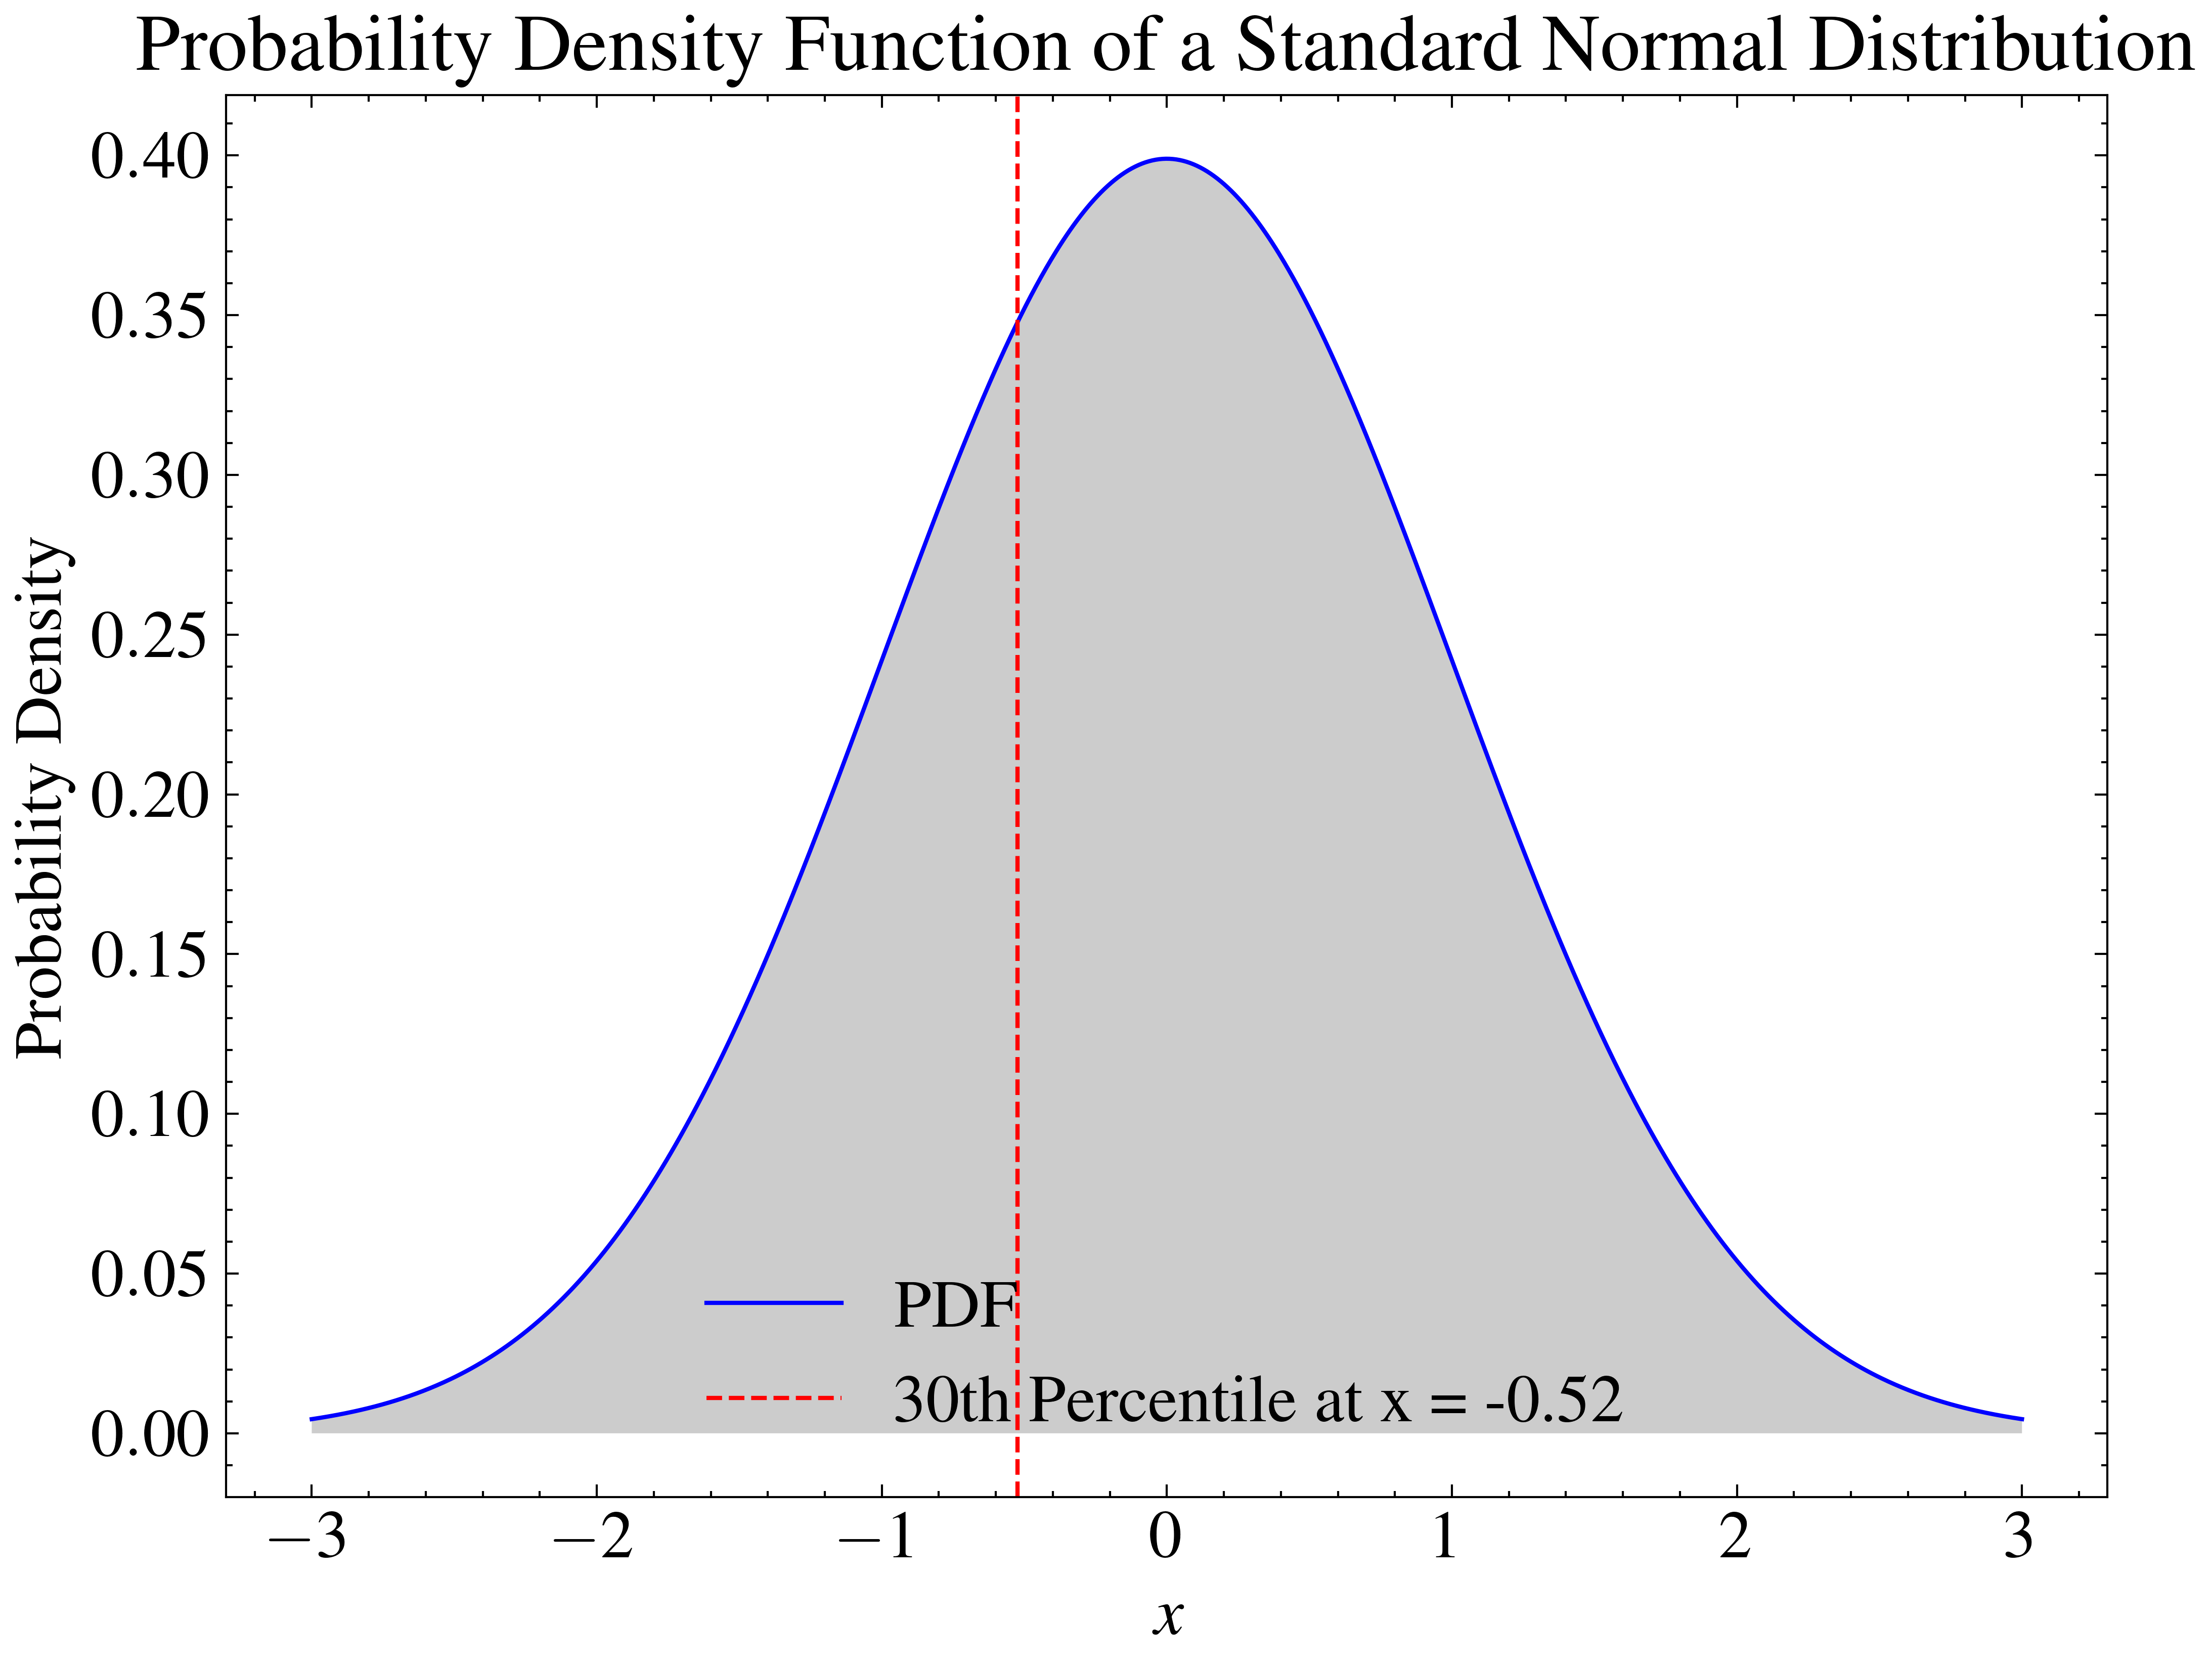
\includegraphics[width=0.8\linewidth]{src/figures/pdf-cdf-quantile/pdf-quantile.png}
        \subcaption{PDF and Quantile}
    \end{subfigure}
    \begin{subfigure}{0.48\columnwidth}
        \centering
        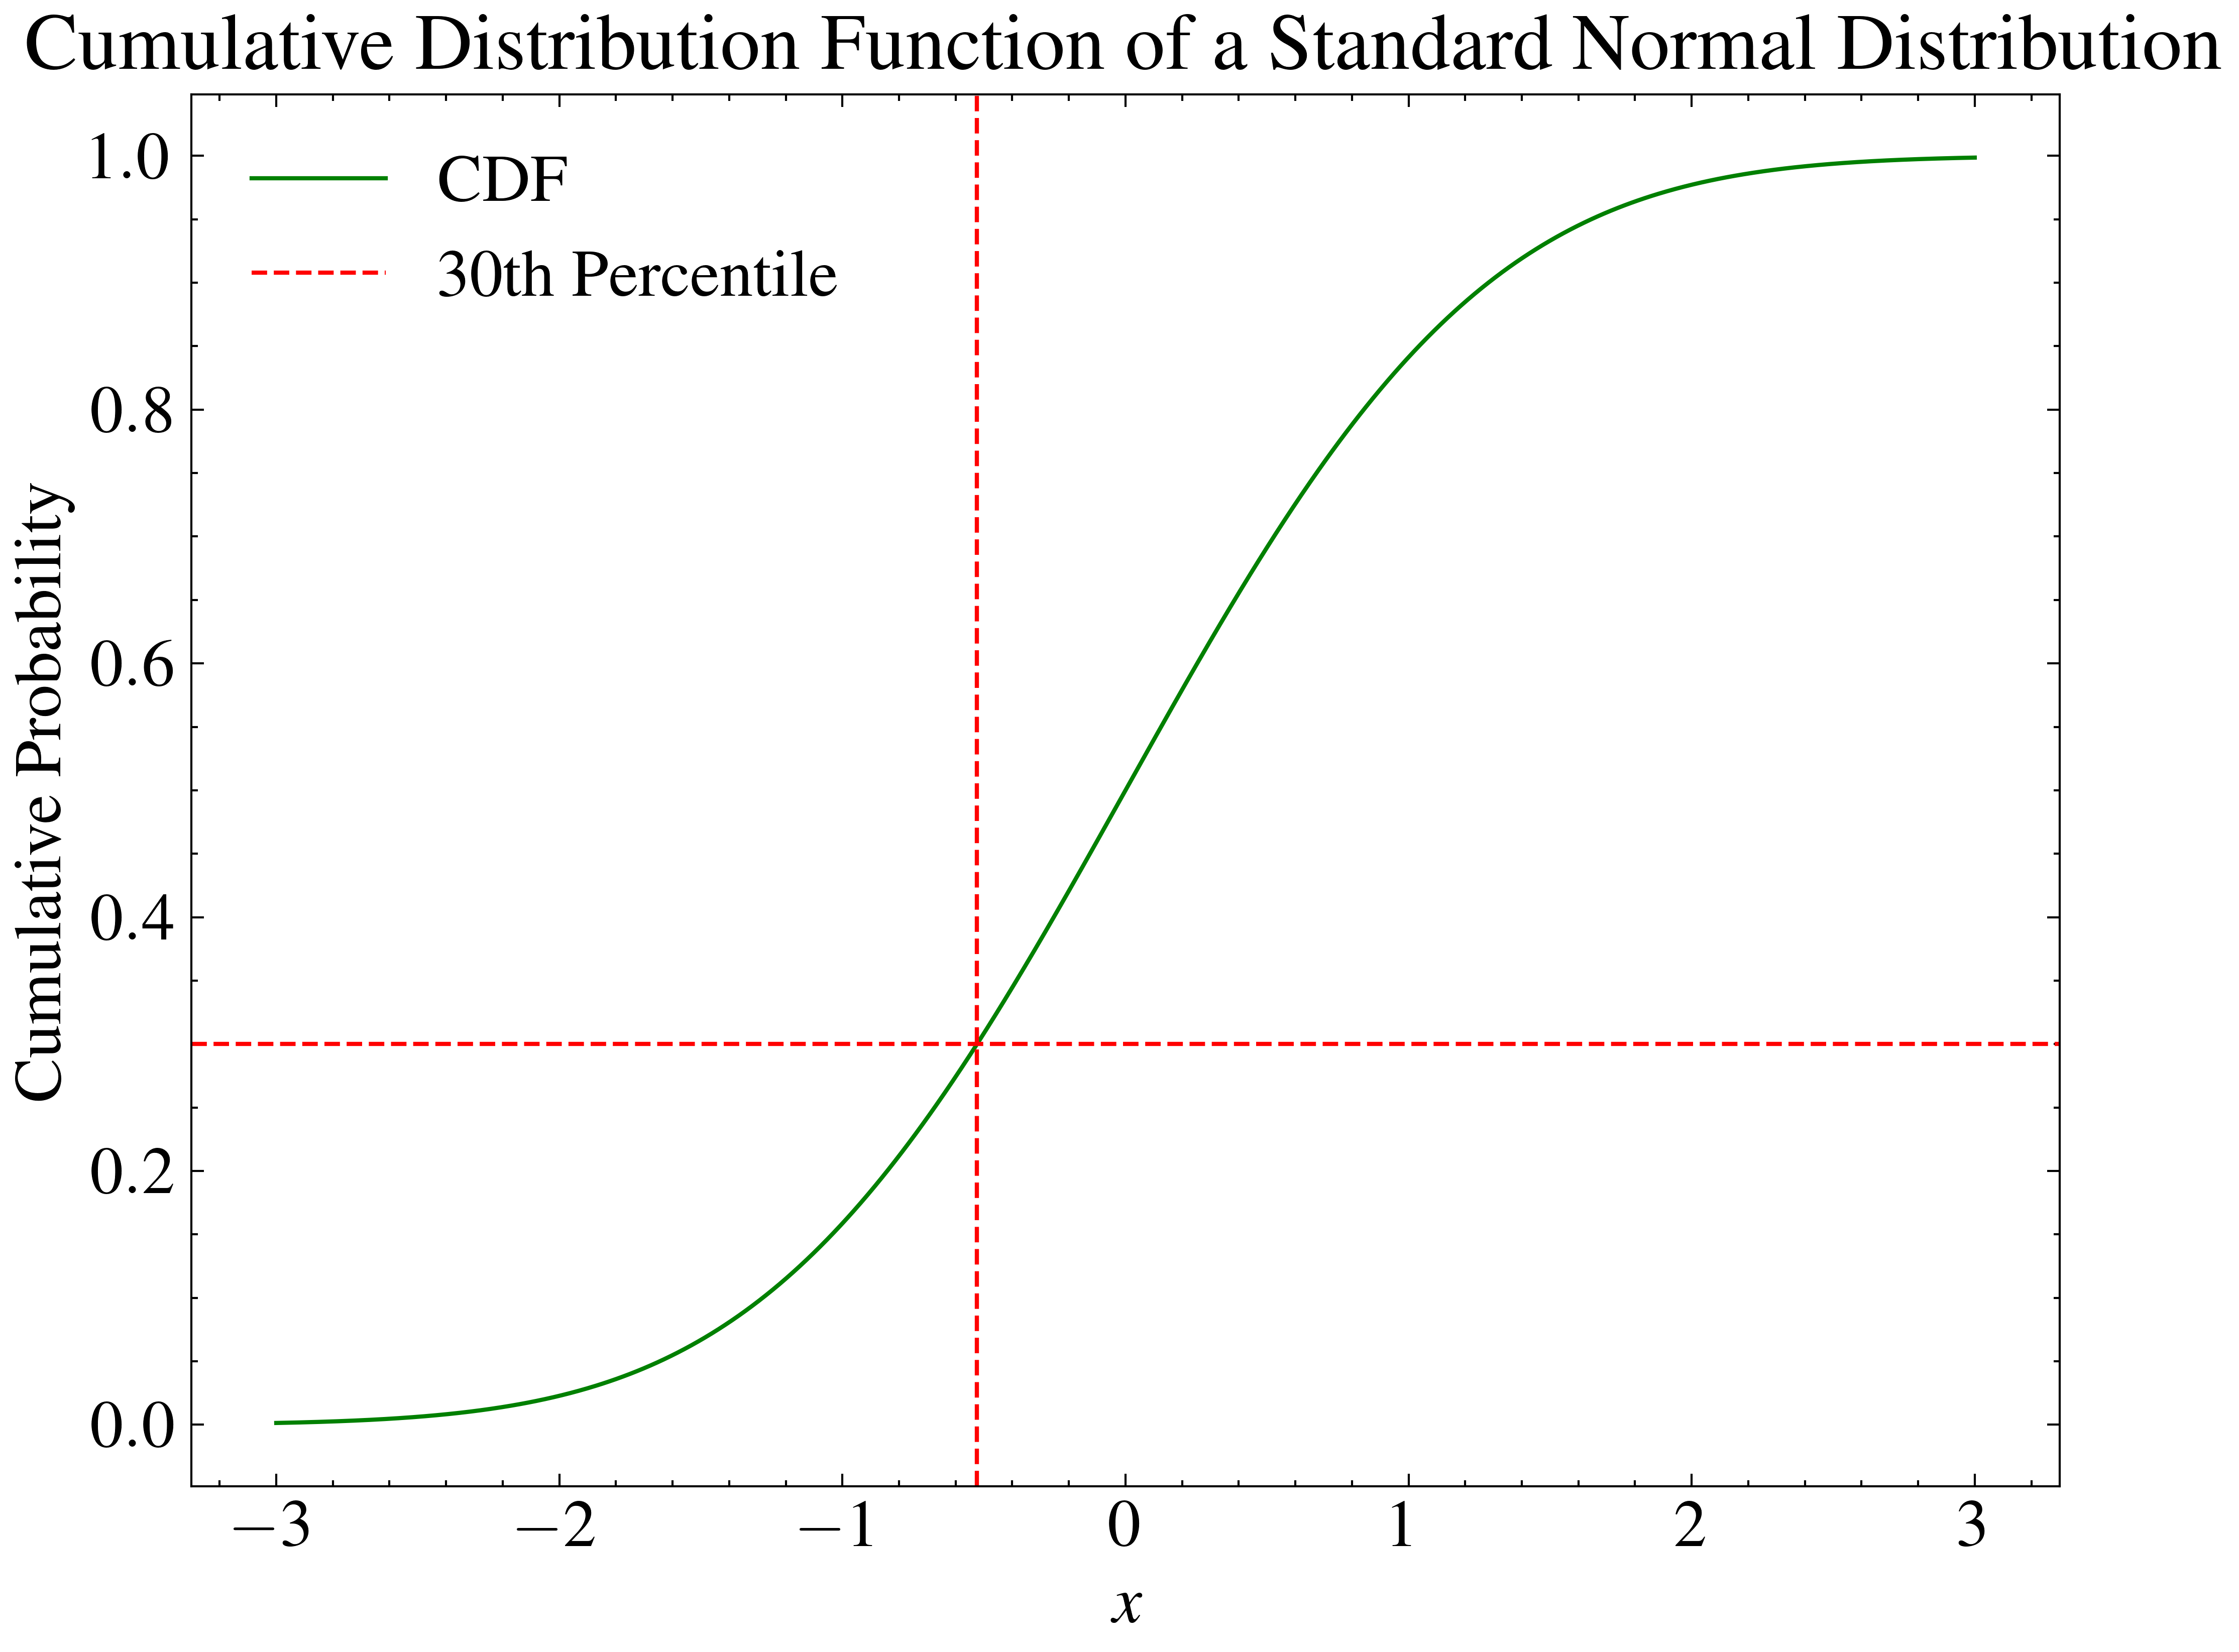
\includegraphics[width=0.8\linewidth]{src/figures/pdf-cdf-quantile/cdf-quantile.png}
        \subcaption{CDF and Quantile}
    \end{subfigure}
    \caption{PDF, CDF and Quantile}\label{fig:pdf-cdf-quantile}
\end{figure}



\clearpage
\subsection{乱数}

\subsubsection{一様乱数}
一様分布に従う乱数のこと。
一様分布のPDF、CDF、Quantileを図\ref{fig:uniform-pdf-cdf}に示す。
\begin{figure}
	\centering
	\begin{subfigure}{0.48\columnwidth}
		\centering
		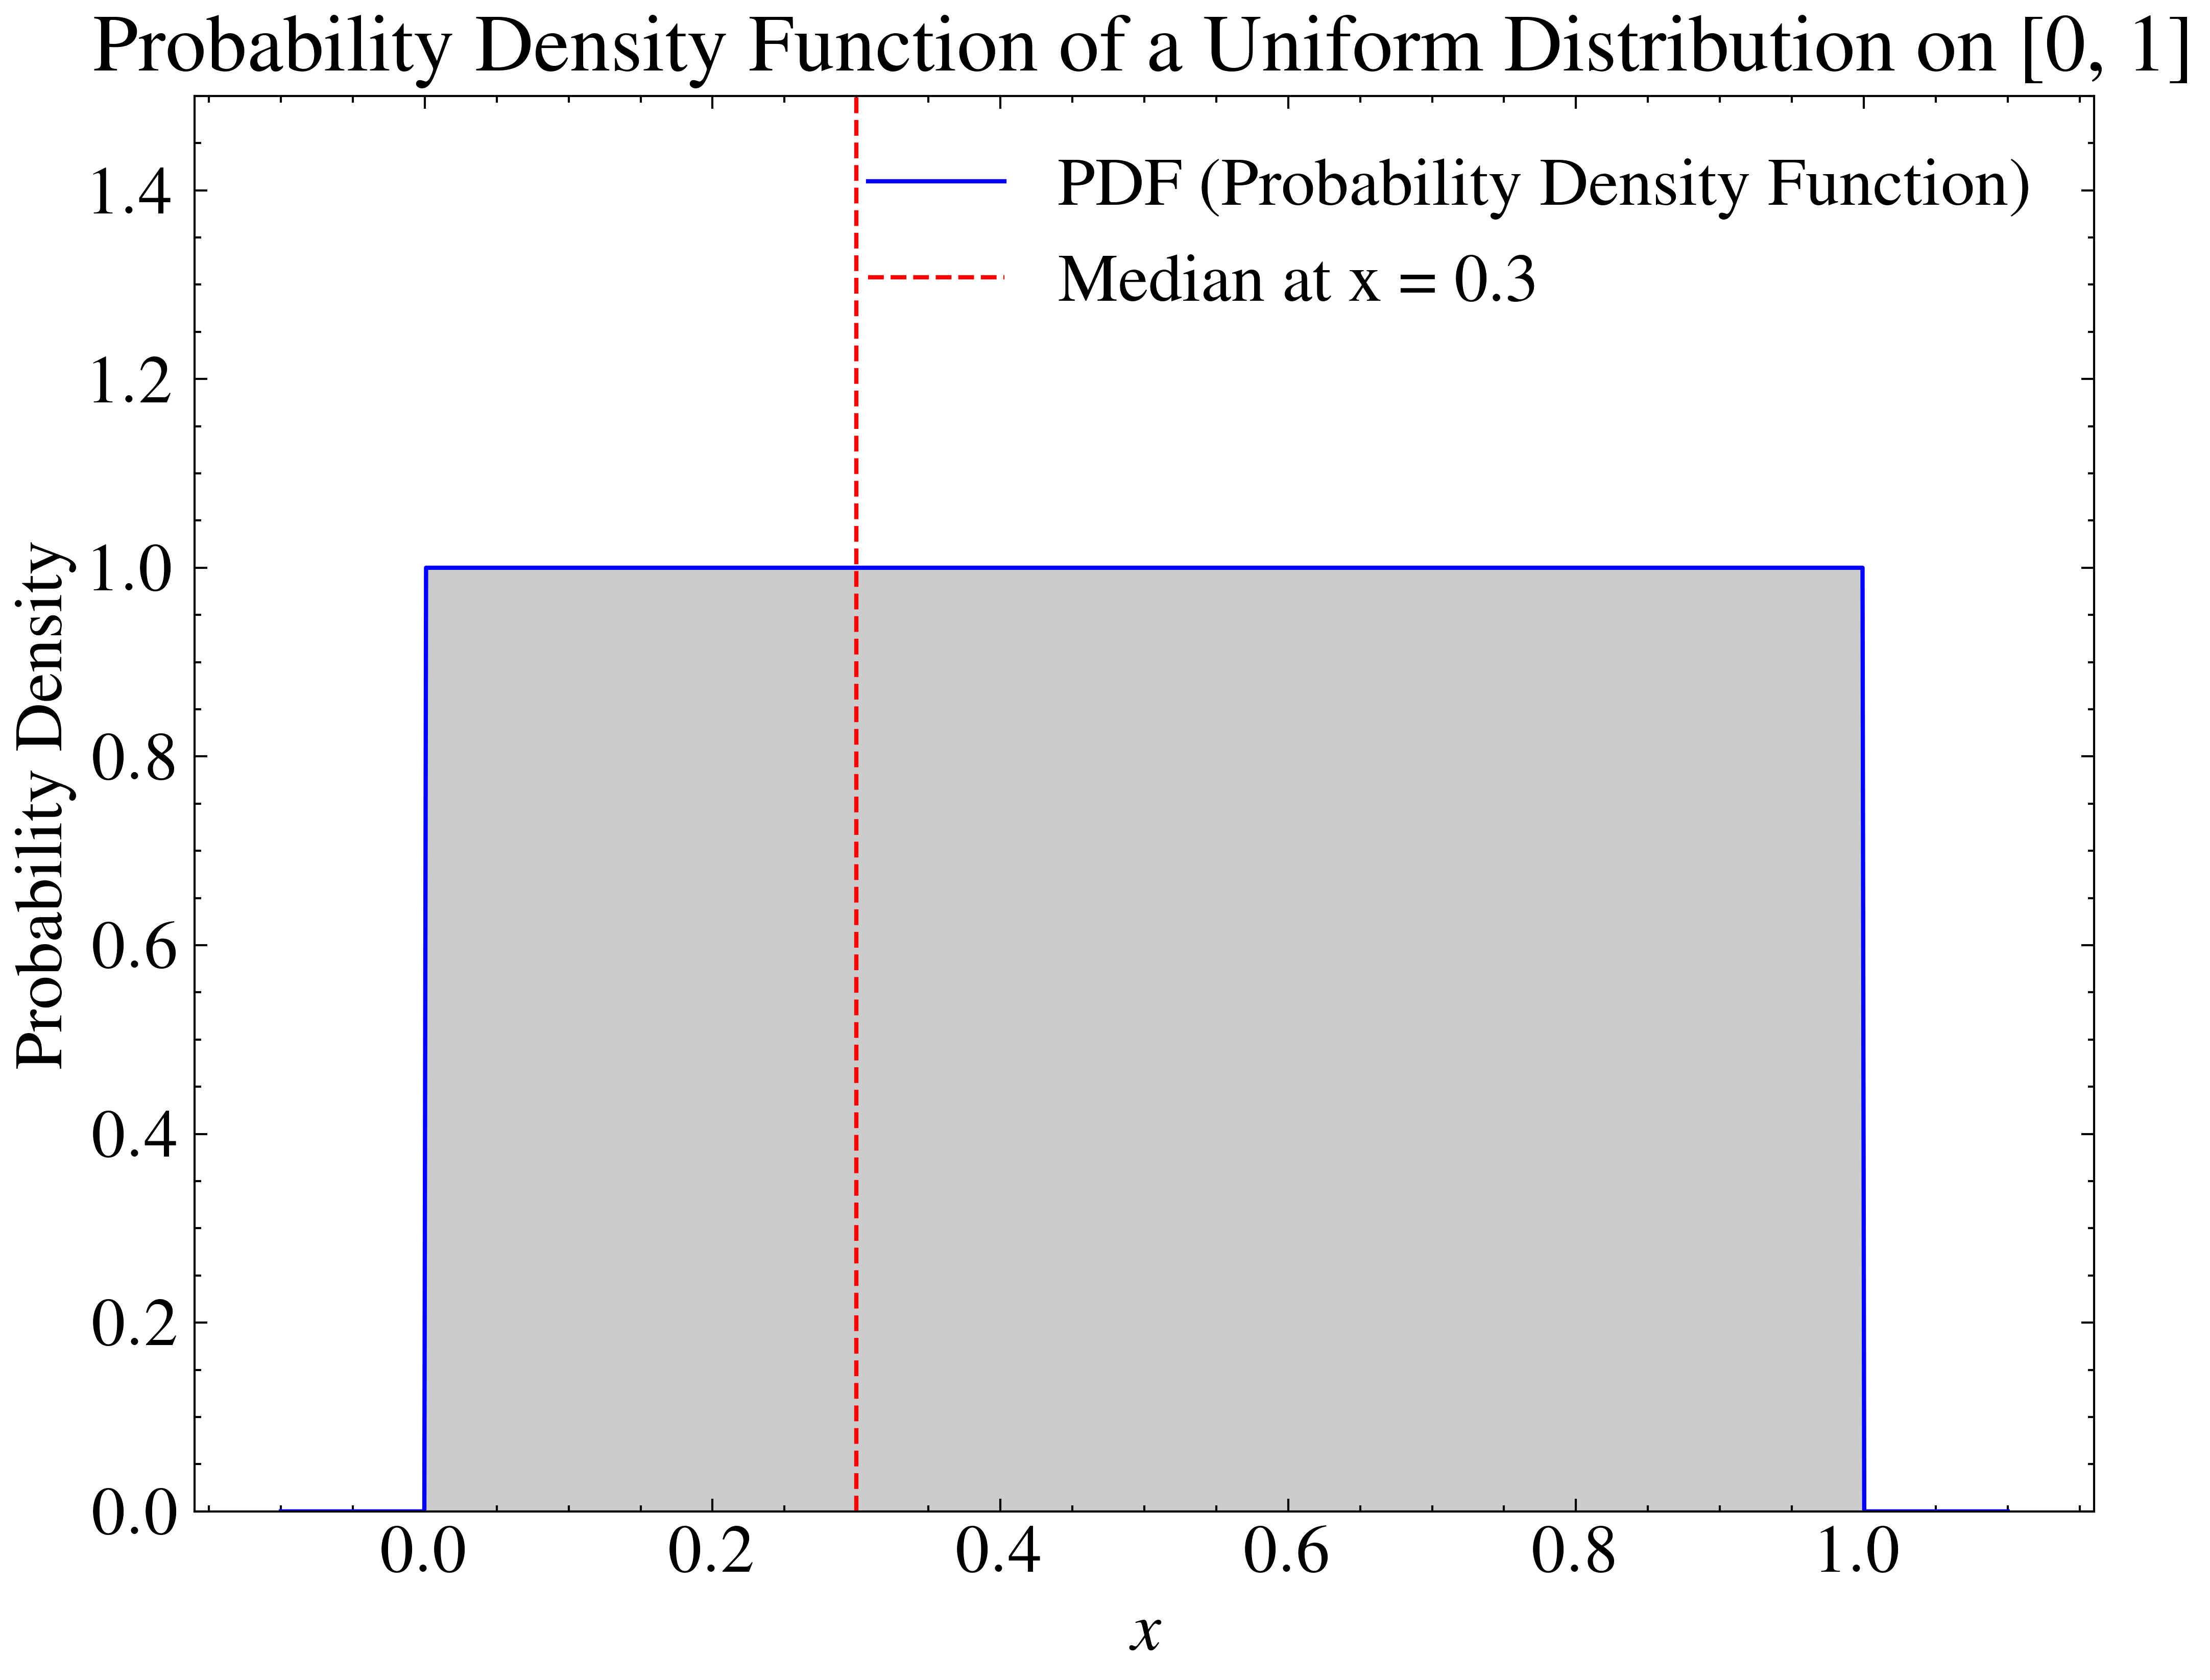
\includegraphics[width=0.8\linewidth]{src/figures/uniform-distribution-pdf-cdf-quantile/uniform_pdf.png}
		\subcaption{PDF}
	\end{subfigure}
	\begin{subfigure}{0.48\columnwidth}
		\centering
		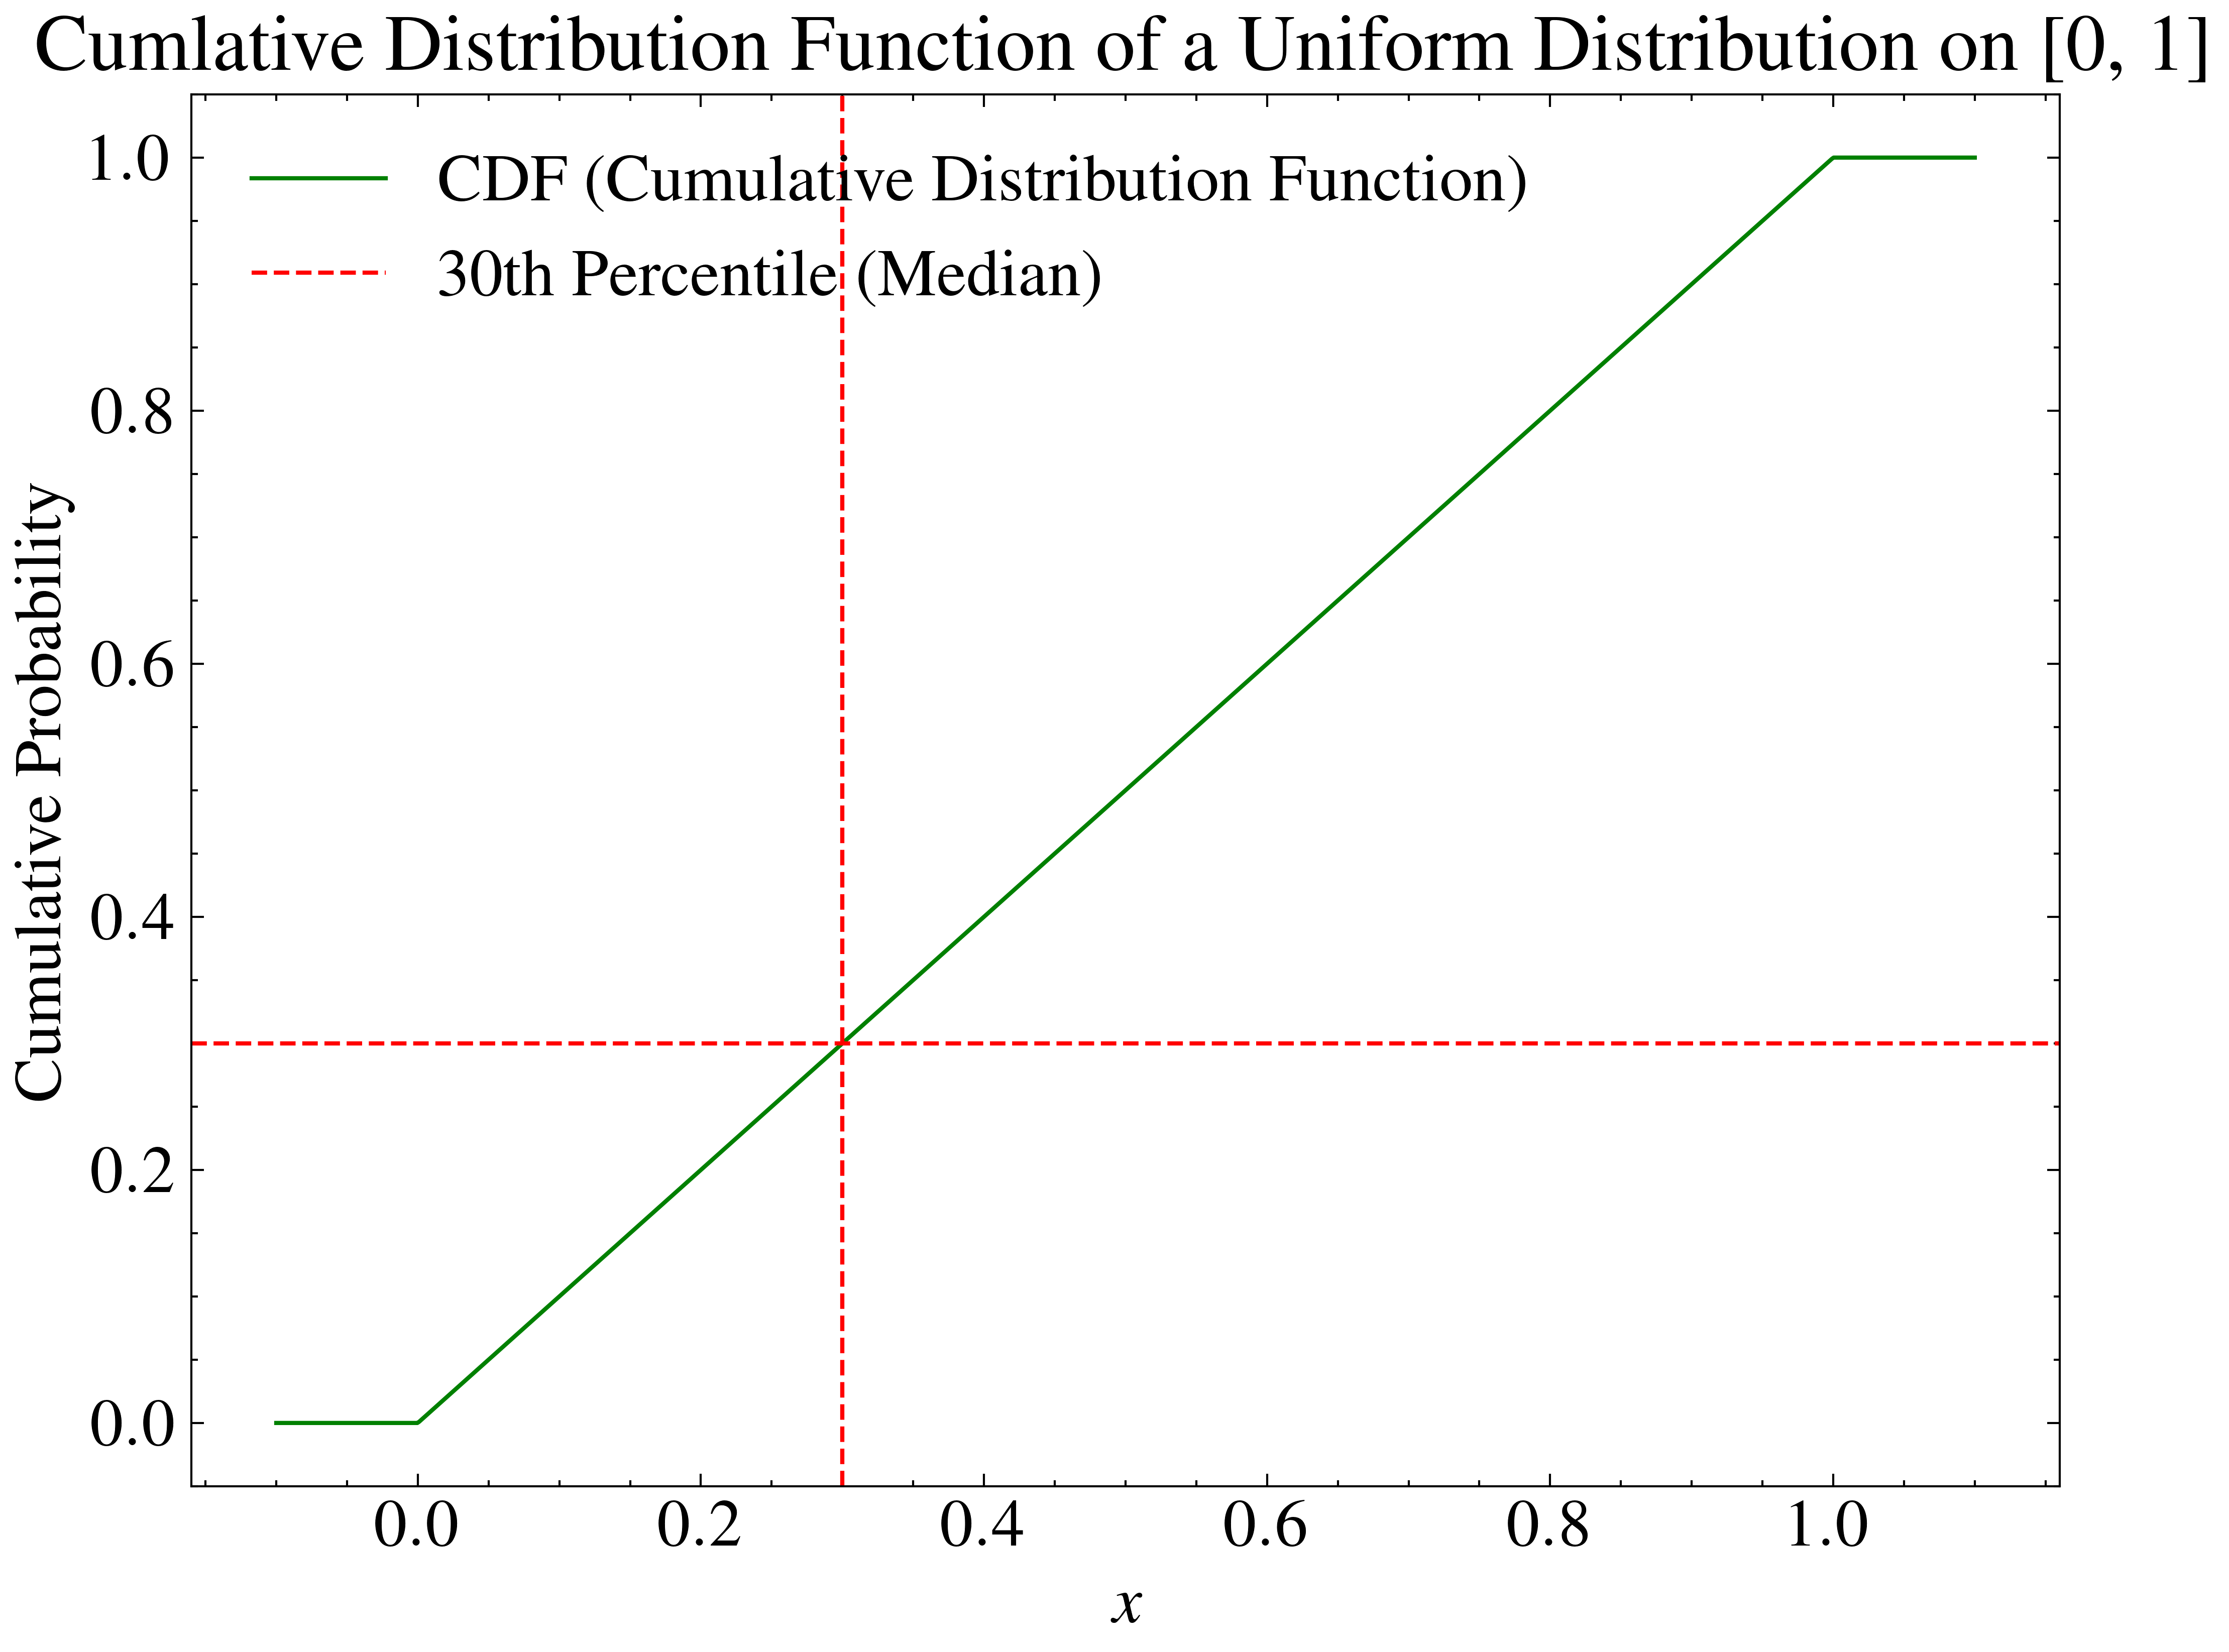
\includegraphics[width=0.8\linewidth]{src/figures/uniform-distribution-pdf-cdf-quantile/uniform_cdf.png}
		\subcaption{CDF}
	\end{subfigure}
	\caption{一様分布のPDFとCDF}\label{fig:uniform-pdf-cdf}
\end{figure}

一様乱数を生成するプログラムは数多く開発されてきたが、中でも最も早い時期に提案された方法が線形合同法である。
線形合同法は、次の漸化式
\begin{equation*}
	X_{n+1} = (aX_n + c) \mod m \,, n = 0, 1, 2, \ldots
\end{equation*}
を用いて、乱数列$X_0, X_1, X_2, \ldots$を生成する方法である。
この漸化式で表される乱数列は周期性をもち、それを長くするために$m$はできるだけ大きくとるのが普通である。
その結果、計算速度が遅くなり実用的でなくなった。

\subsubsection{正規乱数}
正規分布に従う乱数のこと。
正規分布は、平均$\mu$、分散$\sigma^2$の2つのパラメータで特徴づけられ、
\begin{equation*}
	\mathcal{N}(x) = \frac{1}{\sqrt{2\pi}\sigma} \exp\left(-\frac{(x-\mu)^2}{2\sigma^2}\right)
\end{equation*}
と表される。
特に、平均が0、分散が1の正規分布を標準正規分布と呼び、
\begin{equation}
	\mathcal{N}(x) = \frac{1}{\sqrt{2\pi}} \exp\left(-\frac{x^2}{2}\right)
\end{equation}
で表される。
この標準正規分布のPDF、CDF、Quantileは図\ref{fig:pdf-cdf-quantile}に示す。

\paragraph{逆関数法}
乱数変換のための一般的な方法である。
$F(x)$の逆関数
\begin{equation*}
	F^{-1}(y) = \inf\{x: F(x) \geq y \},\, 0 \leq y \leq 1
\end{equation*}
を用いて、
\begin{equation}\label{eq:inverse-function}
	X = F^{-1}(U)
\end{equation}
とすると、
\begin{equation*}
	\mathrm{Pr}\{X \leq x\} = \mathrm{Pr}\{F^{-1}(U) \leq x\} = \mathrm{Pr}\{U \leq F(x)\} = F(x)
\end{equation*}
となり、$X$は$F(x)$に従う乱数となる。


\paragraph{Box-Muller法}
Box-Muller法は、一様乱数を用いて正規乱数を生成する方法である。
具体的には、$[0, 1]$上の一様乱数$U_1, U_2$を用いて、
\begin{equation}\label{eq:box-muller}
	\begin{split}
		Z_1 & = \sqrt{-2\ln U_1} \cos(2\pi U_2) \\
		Z_2 & = \sqrt{-2\ln U_1} \sin(2\pi U_2)
	\end{split}
\end{equation}
とすると、$Z_1, Z_2$は独立な標準正規乱数となる。
以下に簡単な証明を示す。
まず、指数分布と一様分布で正規分布が得られることを示す。
$R$が$[0, 2]$の指数分布に従い、$\Theta$が$[0, 2\pi]$の一様分布に従うとし、
$Z_1 = \sqrt{R}\cos\Theta$、$Z_2 = \sqrt{R}\sin\Theta$とする。
$f$を$Z_1, Z_2$の同時確率密度関数、$g$を$R, \Theta$の同時確率密度関数とすると、
\begin{equation*}
	\begin{split}
		 & \text{$R$が$[0, 2]$の指数分布に従い、$\Theta$が$[0, 2\pi]$の一様分布に従う}                                \\
		 & \Leftrightarrow g(r, \theta) = \dfrac{1}{2\pi} \dfrac{1}{2} e^{-\frac{r}{2}}            \\
		 & \Leftrightarrow f(z_1, z_2) = \dfrac{1}{2\pi} \dfrac{1}{2} e^{-\frac{z_1^2 + z_2^2}{2}} \\
		 & \Leftrightarrow \text{$X_1$と$X_2$は独立な標準正規分布に従う}
	\end{split}
\end{equation*}
となる。
よって二つの独立な標準正規乱数$U_1, U_2$から、
\begin{equation*}
	\begin{split}
		R = -2\ln U_1 \\
		\Theta = 2\pi U_2
	\end{split}
\end{equation*}
とすれば、$Z_1, Z_2$は独立な標準正規乱数となる。


\subsubsection{中心極限定理}
中心極限定理とは、独立な確率変数$X_1, X_2, \ldots, X_n$が同一の分布に従うとき、
その和$S_n = X_1 + X_2 + \cdots + X_n$は$n$が大きくなるにつれて正規分布に近づくという定理である。

まず特性関数を定義する。ある確率変数$X$の特性関数$\varphi(t)$は、
\begin{equation}
    \begin{split}
        \varphi(t) & = \mathrm{E}[e^{itX}]                     \\
                   & = \int_{-\infty}^{\infty} e^{itx} f(x) dx
    \end{split}
\end{equation}
で定義される。
これは、$f(x)$の逆フーリエ変換で、その逆変換
\begin{equation}
    f(x) = \frac{1}{2\pi} \int_{-\infty}^{\infty} e^{-itx} \varphi(t) dt
\end{equation}
が存在する。\footnote{
    つまり、$\varphi(x)$がもとまれば、$f(x)$がもとまることになる。
}
$X$が正規分布$\mathcal{N}(0, \sigma^2)$に従うとき、
\begin{equation}\label{eq:standard-normal-characteristic-function}
    \varphi(t) = e^{-\frac{\sigma^2t}{2}}
\end{equation}

さて、$X_1, X_2, \ldots, X_n$が独立で同一の分布に従うとき、
\begin{equation}
    T_N = \dfrac{1}{\sqrt{n}} \sum_{i=1}^{n} (x_i - \bar{x})
\end{equation}
とおくと、$T_N$の特性関数は
\begin{align*}
    \varphi_{T_N}(t) & = \mathrm{E}\left[e^{itT_N}\right]                                                                                                                  \\
                     & = \prod_i \mathrm{E}\left[\exp{it\dfrac{1}{\sqrt{N}}(x_i - \bar{x})}\right]                                                                         \\
                     & = \left\{\mathrm{E}\left[\exp\left(it\dfrac{1}{\sqrt{N}}\left(x_i - \bar{x}\right)\right)\right]\right\}^n                                          \\
                     & = \left[1 + \dfrac{it}{\sqrt{N}} \mathrm{E}(x - \bar{x}) - \dfrac{t^2}{2N} \mathrm{E}(x - \bar{x})^2 + O\left(\dfrac{1}{N\sqrt{N}}\right) \right]^N \\
                     & = \left[1 - \dfrac{t^2}{2N}\mathrm{V}(X) + o\left(\dfrac{1}{N\sqrt{N}}\right)\right]^N
\end{align*}
となる。
ただし、$\mathrm{E}(x - \bar{x}) = 0$、$\mathrm{V}(X) = \mathrm{E}(x - \bar{x})^2$である。
$N$が十分大きい時、
\begin{align}
    \varphi_{T_N}(t) & = \left( 1 - \dfrac{t^2}{2n}\mathrm{V}(X) \right)^n \nonumber \\
                     & = e^{-\dfrac{t^2}{2}\mathrm{V}(X)}
\end{align}
これは上記の正規分布の特性関数\ref{eq:standard-normal-characteristic-function}式と一致し、
$T_N$は$\mathcal{N}(0, \mathrm{V}(X))$正規分布に従うことがわかる。
これを中心極限定理という。


\clearpage
\subsection{最小二乗法(単回帰)}

ある2変数$x,y$が与えられ、これらの間に比例関係
\begin{equation}\label{eq:linear}
	y = ax + b
\end{equation}
という関係があると予想されるとする。
実験などでは$x,y$に誤差が含まれ全ての$x,y$が\ref{eq:linear}式を満たすような係数$a,b$は存在しない。
このようなとき、しばしば最小二乗法によって係数$a,b$を求める。
最小二乗法は、$n$個のデータ点$(x_i,y_i)$が与えられたとき、
実際の値$y_i$と予測値$ax_i+b$の差の二乗和が最小となるような係数$a,b$を求める方法である。
すなわち、二乗和
\begin{equation}\label{eq:least-square}
	L(a,b) = \sum_{i=1}^{n} (y_i - ax_i - b)^2
\end{equation}
を最小にするような係数$a,b$を求める。
\ref{eq:least-square}式を$a,b$について偏微分し、それぞれの微分が0となるような$a,b$を求めると、
\begin{equation}\label{eq:normal-equation}
	\begin{split}
		 & \pdv{L(a, b)}{a}                                                               = 0              \\
		 & \Leftrightarrow   \left( \sum_i x_i  \right) b + \left(\sum_i x_i^2 \right) a  = \sum_i x_i y_i \\
		 & \pdv{L(a, b)}{b}                                                                                \\
		 & \Leftrightarrow nb + \left( \sum_i x_i \right) a = \sum_i y_i
	\end{split}
\end{equation}
という連立方程式が得られ、これを正規方程式(normal equation)という。
これを解くと、
\begin{equation}\label{eq:regression-equation}
	\begin{split}
		a & = \dfrac{\left(\sum x_i\right)\left(\sum y_i\right) - n\sum x_i y_i}{\left(\sum x_i \right)^2 - n \sum x_i^2} \\
		  & = \dfrac{n \bar{x}\bar{y} - \sum_i x_iy_i}{\bar{x}^2 - \sum x_i^2}                                            \\
		b & = \dfrac{\sum y_i - a\sum x_i}{n}                                                                             \\
		  & = \bar{y} - a\bar{x}
	\end{split}
\end{equation}
となる。
ここで、$\bar{x},\bar{y}$はそれぞれ$x,y$の平均値である。
これら$a,b$による式$y=ax+b$を$y$の$x$上への回帰方程式あるいは回帰直線、$a$を偏回帰係数という。

$b$と相関係数$r=\dfrac{\sum_i (x_i - \bar{x})(y_i - \bar{y})}{\sqrt{\sum_i (x_i - \bar{x})^2 \sum_i (y_i - \bar{y})^2}}$には、
\begin{equation}
	b = r \dfrac{\sqrt{\sum \left(y_i - \bar{y}\right)^2}}{\sqrt{\sum \left(x_i - \bar{x}\right)^2}}
\end{equation}
なる関係があり、また実際の値$y_i$と予測値$\hat{y_i}$の差の二乗和について、
\begin{equation}
	\sum_i d_i^2 \equiv \sum_i \left(y_i - \hat{y_i}\right)^2 = \left(1 - r^2\right) \sum_i \left(y_i - \bar{y}\right)^2
\end{equation}
なる関係がある。
すなわち、$r$は直線の当てはまりの良さを示す指標であり、独立変数\footnote{
	説明変数とも呼ばれる
}
が$x$が、従属変数\footnote{
	非説明変数とも呼ばれる
}
$y$を決定する強弱の度合いを表すため、$r^2$を決定係数と呼ばれる。

\subsection{重回帰分析}
独立変数が一つの場合を拡張し、独立変数が$x_1, x_2, \dots, x_p$と$p$個ある場合を考える。
独立変数が一つの場合の単回帰分析に対して、複数ある場合を重回帰分析という。\footnote{
	単回帰分析では、$x$に対して$y=a+bx$と$y$が決まる状況を考えた。
	これは、2次元で$y$を説明するような直線を考えることになる。
	一方、重回帰分析では、$x_1, \dots, x_p$に対して$y=b_0 + b_1x_1 + \dots + b_px_p$と$y$が決まる状況を考える。
	すなわち、$p+1$次元において、$y$を説明するような(超)平面を考えることになる。
}
いま、$n$個のデータ点$(x_{i1}, x_{i2}, \dots, x_{ip}, y_i)$ $(i=1,\dots,n)$が与えられたとき、最小二乗法を考える。
ベクトル表記を用いて、
\begin{align}
	\bm{y} & = \begin{pmatrix}
		           y_1    \\
		           y_2    \\
		           \vdots \\
		           y_n
	           \end{pmatrix}                             &
	\bm{X} & = \begin{pmatrix}
		           1      & x_{11} & x_{12} & \dots  & x_{1p} \\
		           1      & x_{21} & x_{22} & \dots  & x_{2p} \\
		           \vdots & \vdots & \vdots & \ddots & \vdots \\
		           1      & x_{n1} & x_{n2} & \dots  & x_{np}
	           \end{pmatrix} &
	\bm{b} & = \begin{pmatrix}
		           b_0    \\
		           b_1    \\
		           b_2    \\
		           \vdots \\
		           b_p
	           \end{pmatrix}
\end{align}
とすると、$\bm{b}$による予測値$\bm{\hat{y}}$は、
\begin{equation}\label{eq:regression-multiple}
	\bm{\hat{y}} = \begin{pmatrix}\hat{y_1}\\ \hat{y_2} \\ \vdots \\ \hat{y_n}\end{pmatrix} = \bm{Xb}
\end{equation}
とかける。
最小にすべき二乗和は、
\begin{equation}\label{eq:least-square-multiple}
	\begin{split}
		L(\bm{b}) & = \| \bm{y}  - X\bm{b} \|^2                                                                     \\
		          & = \trans{\bm{y}} \bm{y} - 2 \trans{\bm{b}} \trans{X} \bm{y} + \trans{\bm{b}} \trans{X} X \bm{b}
	\end{split}
\end{equation}
とかける。\footnote{
	$\trans{\bm{b}}\trans{X}\bm{y}$はスカラーであるから、転置をとっても変わらない。
	$\trans{\bm{b}}\trans{X}\bm{y} = \trans{\bm{y}}X\bm{b}$である。
}
求める$\bm{b}$は、$L(\bm{b})$の勾配ベクトルが$\bm{0}$となるような$\bm{b}$であるから、
\begin{equation}\label{eq:normal-equation-multiple}
	\begin{split}
		\grad{L(\bm{b})} & = -2\trans{X}\bm{y} + 2\trans{X}X\bm{b} = 0 \\
		\Leftrightarrow  & \trans{X}X\bm{b} = \trans{X}\bm{y}
	\end{split}
\end{equation}
とかける。\footnote{
	$\grad{\trans{\bm{b}}\trans{X}\bm{y}} = \trans{X}\bm{y}$、
	$\grad{\trans{\bm{b}}\trans{X}X\bm{b}} = 2\trans{X}X\bm{b}$であることを用いた。
	後者は二次形式と呼ばれる形である。
}
この解を$\bm{\hat{b}}$と書き、\ref{eq:least-square-multiple}式を最小にする$\bm{b}$である。

$\bm{y}$の偏差の二乗和$S_{\bm{y}}^2$は、
\begin{align}\label{eq:y-deviation}
	S_{\bm{y}}^2 & = \| \bm{y} - \bm{\bar{y}} \|^2 \nonumber                                                                                                                         \\
	             & = \trans{\left\{ (\bm{y}-\bm{\hat{y}}) + (\bm{\hat{y}} - \bm{\bar{y}}) \right\}} \left\{  (\bm{y}-\bm{\hat{y}}) + (\bm{\hat{y}} - \bm{\bar{y}})\right\} \nonumber \\
	             & = \| \bm{\hat{y}} - \bm{\bar{y}} \|^2 + \| \bm{y} - \bm{\hat{y}}^2 \|
\end{align}
とかける。
ここで、\ref{eq:normal-equation-multiple}式を変形し、\ref{eq:regression-multiple}式を代入すると
\begin{equation}
	\begin{split}
		 & \trans{X} \left( \bm{y} - X\bm{b} \right) = \trans{X} \left( \bm{y} - \bm{\hat{y}} \right) = 0 \\
		 & \Leftrightarrow \trans{\bm{b}}\trans{X} \left( \bm{y} - \bm{\hat{y}} \right) = 0               \\
		 & \Leftrightarrow \trans{\bm{\hat{y}}} \left( \bm{y} - \bm{\hat{y}} \right) = 0                  \\
	\end{split}
\end{equation}
となることと、\ref{eq:regression-multiple}式で第一列に注目すると、
\begin{equation}
	\begin{split}
		 & \begin{bmatrix}1 & 1 & \dots & 1 \end{bmatrix}
		(\bm{y} - \bm{\hat{y}}) = 0                                         \\
		 & \Leftrightarrow \trans{\bm{\bar{y}}} (\bm{y} - \bm{\hat{y}}) = 0
	\end{split}
\end{equation}
となることを用いた。
\ref{eq:y-deviation}式は、$S_{\bm{y}}^2$が前半部分の$X$による部分と後半部分の$X$で説明されない部分に分かれ、$S_{\bm{y}}^2 = S_{\bm{\hat{y}}^2} + L(\bm{b})$と書ける。
そして、この$X$によって説明される部分の割合を決定係数と呼び、
\begin{align}
	R^2 & = \dfrac{S_{\bm{\hat{y}}}^2}{S_{\bm{y}}^2} = \dfrac{\| \bm{\hat{y}} - \bm{\bar{y}} \|^2}{\| \bm{y} - \bm{\bar{y}} \|^2} \\
	    & = \dfrac{S_{\bm{y}}^2  - L(\bm{b})}{S_{\bm{y}}^2} \nonumber                                                             \\
	    & = 1 - \dfrac{L(\bm{b})}{S_{\bm{y}}^2}
\end{align}
と定義される。


\end{document}
